\begin{figure}[t]
  \centerline{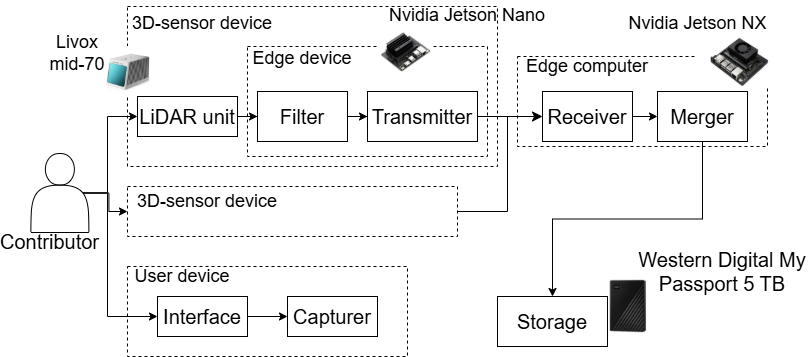
\includegraphics[width=\linewidth]{img/experiment_system.png}}
  \caption{Experiment system}
  \label{exp_system}
\end{figure}

\begin{figure}[t]
  \centerline{\includegraphics[width=\linewidth]{img/dyployment_site.png}}
  \caption{Experimental site}
  \label{exp_site}
\end{figure}

Fig.~\ref{exp_system} shows our experimental system based on Fig.~\ref{systemmodel}.
The experimental system consisted of multiple 3D-sensor devices, an edge computer, a user device, and storage.
\deleted{Point-cloud data from the sensors are filtered, transmitted, integrated on the basis of timestamps, and stored.}
\revised{Point-cloud data from the sensors were filtered, transmitted, integrated on the basis of timestamps, and stored.}
\deleted{The user device captures activity-level indicators.}
\revised{The user device captured activity level indicators.}
A Livox Mid-70 \cite{Mid70}, NVIDIA Jetson Nano \cite{Jetsonnano}, and NVIDIA Jetson Xavier NX \cite{JetsonNX} were used as the LiDAR unit, edge device, and edge computer, respectively.
Each contributor's laptop served as the user device.
\deleted{The evaluation verifies activity-level estimation from dynamic features extracted from 3D point-cloud data, without optimizing sensor placement or calibration \cite{9789786,10636133}.}
\revised{The evaluation verified activity level estimation from dynamic features extracted from 3D point-cloud data, without optimizing sensor placement or calibration \cite{9789786,10636133}.}
Akiyama et al.\ demonstrated that multiple LiDAR sensors can eliminate blind spots in indoor spaces \cite{9789786}.
\deleted{The present evaluation focuses on dynamic feature effectiveness rather than spatial calibration or sensor-placement optimization.}
\revised{The present evaluation focused on dynamic feature effectiveness rather than spatial calibration or sensor-placement optimization.}
Fig.~\ref{exp_site} shows the experimental site.
The experiment was conducted in lab room, located at the Toyosu Campus of Shibaura Institute of Technology in Koto-ku, Tokyo, Japan.
Each LiDAR unit was placed 1.0 m to the left and right of the center of the user-device keyboard, mounted at a height of 0.15 m using a tripod, tilted 10° horizontally with respect to the desk, and configured to operate at a sensing rate of 110 frames per second.
